\documentclass[conference]{IEEEtran}
\IEEEoverridecommandlockouts
% The preceding line is only needed to identify funding in the first footnote. If that is unneeded, please comment it out.
\usepackage{cite}
\usepackage{amsmath,amssymb,amsfonts}
\usepackage{algorithmic}
\usepackage{graphicx}
\usepackage{textcomp}
\usepackage{xcolor}
\def\BibTeX{{\rm B\kern-.05em{\sc i\kern-.025em b}\kern-.08em
    T\kern-.1667em\lower.7ex\hbox{E}\kern-.125emX}}
\begin{document}

\title{Background and Discussion on Use and Implementation of Deep Learning with FPGA\\
%{\footnotesize \textsuperscript{*}Note: Sub-titles are not captured in Xplore and
%should not be used}
%\thanks{Identify applicable funding agency here. If none, delete this.}
}

\author{\IEEEauthorblockN{1\textsuperscript{st} Dimitri Häring}
\IEEEauthorblockA{\textit{School of Engineering (Electrical Engineering)} \\
\textit{Grand Valley State University}\\
Grand Rapids, MI, United States of America \\
haringd@mail.gvsu.edu}
}

\maketitle

\begin{abstract}
%%%%%%%%%%%%%%%%%%%%%%%%%%%%%%%%%%%%%%%%%%%%%%%%%%%%%%%%%%%%%%%%%%%%%%%%%%%%%%%%%%%%%%%%%%%%%%%
%%    Explanation on how to write an executive Summary (ES) out of EGR 602 Winter 2018      %%
%%%%%%%%%%%%%%%%%%%%%%%%%%%%%%%%%%%%%%%%%%%%%%%%%%%%%%%%%%%%%%%%%%%%%%%%%%%%%%%%%%%%%%%%%%%%%%%	
%      Purpose Statement
%      - Concise, solid & comprehensive
%      Summary of tasks and work performed
%      - Concise & quick.
%      Summary of results found
%      - Concise & quick.
The propose of the paper is to introduce the audience to the background of deep learning with an focus on computational challenges and approaches.

Using advanced searches in the IEEE explorer allowed to gain access to published papers about the researched topics to outline the boundaries of the general concepts that have to be explained, elaborated and discussed. Furthermore, Furthermore, actual newspaper articles as well as free lecturers from Standford university where used to build a knowledge base that allowed the author to boldly go where a lot of engineers have been gone before. In addition, the comparison of multiple sources allowed to gain new knowledge.

Results indicate that the implementation of deep learning with artificial neural network can be used as accelerator and improve energy efficiency significantly.
%This document is a model and instructions for \LaTeX.
%This and the IEEEtran.cls file define the components of your paper [title, text, heads, etc.]. *CRITICAL: Do Not Use Symbols, Special Characters, Footnotes, 
%or Math in Paper Title or Abstract.
\end{abstract}

\begin{IEEEkeywords}
Deep Learning, Artificial Neural Network, Planetary Rover
\end{IEEEkeywords}

\section{Introduction}
This paper is an introduction into deep learning. 
First, an overview is presented with a comparison between machine learning and deep learning. 
This allows readers with less background to follow the reasons why deep learning often is associated with neural networks in particular artificial neural networks. 

Second, computational challenges are discussed in terms of performance and power efficiency are discussed and figures given to give an scene of magnitude of different sizes of neural networks.

Third, computational approaches are discussed by using two examples that differs in complexity and performance.
Therefor, Section \ref{sec: Background} introduces the audience to the necessary background required to understand what machine and deep learning means.
%Deep learning is used in a wide range of applications but especially show improved performance in pattern recognition. Where as image recognition and speech recognition are often used as examples or for testing to show performance improvements if a field programmable gate array (FPGA) is used over a conventional central processing unit (CPU). Furthermore, most often a dedicated FPGA seems to have a better energy performance in comparison to a FPGA. 
%
%Second, deep learning (DL) will be the focus point and especially the different methods that are commonly used as neural networks (NN). 
\section{Background}\label{sec: Background}


\subsection{General Concepts}\label{subsec: General Concepts}
Learning is a commonly used word and means according to Merriam Webster the following \cite{Learning}:
\begin{enumerate}
	\item[] 1 : the act or experience of one that learns\\
	$\backslash\backslash$ a computer program that makes learning fun
	\item[] 2 : knowledge or skill acquired by instruction or study
	$\backslash\backslash$ people of good education and considerable learning
	\item[] 3 : modification of a behavioral tendency by experience (such as exposure to conditioning)
\end{enumerate}
This means that a machine that learns receives either instructions or experiences something. This leads to the not unreasonable assumption that if a machine learns, somebody teaches the machine in form of instructions or exploits the machine to experience. To give  a machine instructions is most likely the essence of the todays computing. While a machine is capable of receiving instructions in many different forms the most common at the time is still the users instruction, according to the authors opinion. By applying this concept to a machine that learns a instruction in terms of machine learning not a single instruction is given a algorithm is implemented that similar to adaptive filtering in signal processing wights an input $x$ and will provide an output $z$. The a function $W$ is used to define the weight according to different methods as example linear regression or a second order polynomial. The issue for such an algorithm is the weighting function $W$ needs to be defined by a human that invests a lot of time studying cases and tries to figure out what might be the best function to weight the input for a certain situation. By introducing this thought of weight which is implemented as a simple multiplication of an input value $x$.  This allows to use a vector to describe inputs hence the weights would be a vector of the same length. Now if as example an image of 128x128 pixels would be wighted a vector of length 16384 would have to be used, assuming it is a chromatic picture with a single integer that defines each pixel. This is a real simple example as you start thinking about it but nobody in the world would try to do that with no strategy on hand. To make a point, a machine would have to learn how to interpret a picture depending on the state of the wight of each pixel or most likely groups of pixels. A machine could improve the resolution of his weighting function by learning known pictures where the result is known which is known as \textbf{supervised learning}. Due to the fact that a machine can learn such sets and define a wight for each situation very fast a machine is capable of learning more situations in days than a human is capable of in years.

At this point lets create a hypothetical scenario to understand learning furthermore. Assume that a human with all cognitive abilities that we have just start to exist on a plane with a river and a sun. As a human needs a lot of water most likely this human would experience a sense of thirstiness at some point. The human has no teacher and no previous knowledge so how can the human know that he can drink from the river if not learned from a teacher.

Assume there is an animal too on this plane that drinks from the water. If there is no teacher and a similar situation and obviously no other option than to explore the river the human might be try to do the same even not knowing that it will help to still the sense of thirstiness. The human \textbf{learned unsupervised} by experience of a situation as a witness.
%Unsupervised Learning

This rises the question would make a human brain the decision that it could try to drink from the river with having a single reference. The authors best guess is that most likely a decision would be either drinking, not drinking or something else not expected like trying to communicate with the animal and ask it why it drinks. This shows that a solution can have more possibilities then just yes or no which can be \textbf{classified} as a vector. 

In summary, there are three important terms to know, highlighted in the previous Section \ref{subsec: General Concepts} which are input, output, supervised learning, unsupervised learning, classification. Notice, this is not meant to be a full list of concepts there is more to explore and to know. Due to the fact that the paper shall not exceed a certain length not every concept is discussed rather than a subset is chosen that seems in the authors opinion the most important to understand the background of the matter. 

The next Section \ref{subsec: Machine Learning} is dedicated to machine learning. 

\subsection{Machine Learning}\label{subsec: Machine Learning}
Where as general concepts has been discussed in the previous section \ref{subsec: General Concepts} in this section machine learning will be discussed. In machine learning all the previous discussed concepts can be applied. As the previous discussed example of an 128x 128 picture introduced the goal is to find functions that wights the input there for in machine learning which involves usually no more then one non linear logic layer that is applied to each input vector. The goal is to optimize the weight function $W$ in case of using the concept of supervised learning it would be a predefined set of pictures with known result that is instructed to machine. A commonly known and widely used set is Caltech 101 \cite{Caltech101}. 

Know most decisions are not based on a simple algorithm or one set of pixels it is usually a combination of those patterns. Due to the fact that humans are not capable of performing complex tasks only simple ones in series or parallel, it might not be the best way to analyze a picture as such. 

Therefor, a artificial neural network is discussed in Section \ref{subsec: Artificial Neural Network}.

\subsection{Artificial Neural Network}\label{subsec: Artificial Neural Network}
As the previous Section \ref{subsec: Machine Learning} discussed briefly machine learning and introduced the process of decisions this section is discussing artificial neural networks (ANN). 

A brain is build with neurons, a single neuron is shown in Figure \ref{fig: neuron1}. According to Merriam Webster a neuron is defined as the following \cite{Neuron}:\\
\begin{enumerate}
	\item[] :  a grayish or reddish granular cell that is the fundamental functional unit of nervous tissue transmitting and receiving nerve impulses and having cytoplasmic processes which are highly differentiated frequently as multiple dendrites or usually as solitary axons which conduct impulses to and away from the cell body : NERVE CELL sense 1
\end{enumerate}
In the authors interpretation this means that a neuron receives a input signal $x$ from another neuron. A neuron outputs a signal $z$ to the next neuron. The neuron does weight the signal with function $W$ by modifying it as shown in Equation \ref{eq: one}.
\begin{equation}
\vec{W}(\vec{x})=\vec{z}\label{eq: one}
\end{equation}
At this point it seams to be appropriate that it is commonly known that the eight function $W$ is a non linear function. The reason is kind of simple if it would be a linear function then you could use Gauss to solve for an equation if the matrices are invertible. However, the point is that the brain does network with a single neuron it works with many neurons each connected to each other in an three dimensional space, which makes it kind of complex at the end.
Therefor, do not try to copy a machine that you do not understand it is not an engineer that will solve the brains complexity most likely it will be an neuron scientist and the engineer will use his research and apply the research to common technology.
\begin{figure}[htbp]
\centerline{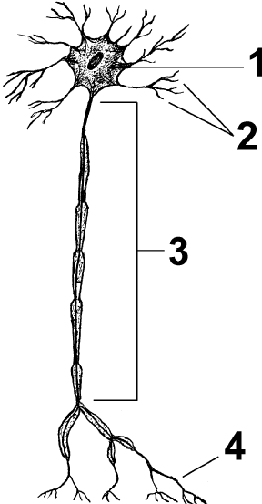
\includegraphics[width=0.2\textwidth]{01_images/neuron1.PNG}}
\caption{Illustration of Neuron: 1 cell body, 2 dendrite, 3 axon, 4 nerve ending \cite{Neuron}.}
\label{fig: neuron1}
\end{figure}
To emphasis the functions of multiple neurons an ANN is build out of multiple non linear  logic layers. Figure \ref{fig: fig_algo_example} shows how one logic layer would look like based on formula presented in Equation \ref{eq: one}. Notice, that in this example not a specific algorithm commonly known is used because the algorithm would be chosen or have been designed to specific problem. By accumulating multiple non linear logic layers to a vast network where as usually each layer is dedicated to a specific task an artificial neural network is build.

Section \ref{subsec: Deep Learning} will discuss the use of neural networks in a field called deep learning.
\begin{figure}[htbp]
	\centerline{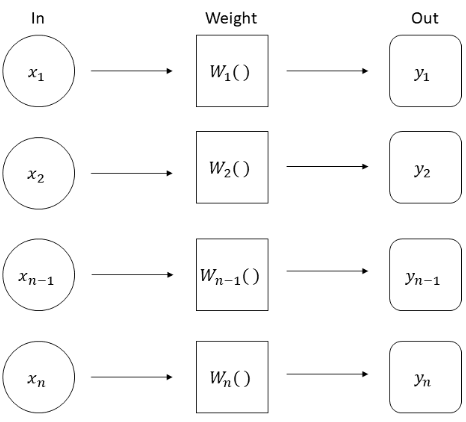
\includegraphics[width=0.45\textwidth]{01_images/fig_algo_example.PNG}}
	\caption{Visualized algorithm of Equation \ref{eq: one}.}
	\label{fig: fig_algo_example}
\end{figure}

\subsection{Deep Learning}\label{subsec: Deep Learning}
As ANN has been discussed in Section \ref{subsec: Artificial Neural Network} this section will provide inside why deep learning is a subset of machine learning. 

As the knowledge has been gathered that an ANN is a cumulation of non liner logic layers and an Machine learning algorithm was defined as a single layer of a non linear logic which determines the main difference between machine learning and deep learning. Deep refers to the number of non linear logic levels that are implied in the ANN. Therefor, Schmidhuber introduced a concept of credit assignment for each stage and depending on the number of credits assigned a distinction between shallow learning and deep learning can be made \cite{Schmidhuber}. Due to the scope of the paper the shallow learning will not be further discussed.

Section \ref{sec: Computational challenges} will provide a deeper inside to specific applications where deep learning is applied in combination with an FPGA to accelerate process speed and energy efficiency.

\section{Computational challenges}\label{sec: Computational challenges}
As discussed in Section \ref{subsec: Deep Learning} deep learning uses in general a form of an ANN. In this section discuss why it is useful to use an FPGA for the ANN implementation.

As discussed each layer of an ANN represents an weighting function so that in general one layer could be reduced to the thought of an flip-flop of an shift register. Each time the shift register shifts the information trough the layers more information about the input will be gathered by applying different methods. As we can identify that each layer has similar patterns to general logic it makes sense to implement it on an FPGA platform. Hedge et. al \cite{Hegde} performed performance measurements for different supervised learning sets, to name one Caltech101 \cite{Caltech101}. To implement the neural network (NN)  the team used an MXP-enhanced FPGA platform because it delivers 1.4-5x higher energy efficiency than all other platforms.  Furthermore, the supervised learning sets where run on a GPU, CPU, and DSP platform.

Gankidi et. al \cite{Gankidi} discusses in his work FPGA Architecture for deep learning and its application to planetary robotics where the problem of constrained embedded system and the power efficiency is considered critical. The comparison between an i5 2.3 GHz CPU and an Xilinx-Space-garde Virtex FPGA is made in terms of energy performance. As introduction Gankidi et. al provides also interesting figures to clarify the need for FPGA architecture on constrained devises by stating that Google brain uses around 16,000 CPUs and consumes around 5 MW of power. While in comparison an a planetary rower with an radiation hardened processor RAD750 uses 5 W of power which differs in the magnitude of $10^6$ in power consumption. This clearly states that there are boundaries to computing and paramount challenges to implement a big enough ANN onto a continent embedded systems. Therefore an FPGA could significantly enhance performance depending on the algorithm and task it is assigned for.

Section \ref{sec: Computational approaches} will discuss an approach of an implemented convolution neural network on FPGA. 

\section{Computational approaches}\label{sec: Computational approaches}
As Section \ref{sec: Computational challenges} introduced performance advantages of the FPGA platforms other other architectures this section will focused on two applied examples on how to implement deep learning ANN on FPGA architecture.

Bacis et. al \cite{Bacis} used a pipelined and scalable dataflow implementation of convolutional neural networks on FPGA with ANN for image classification and image recognition. The convolutional neural network structure is shown in Figure \ref{fig: Convolutional_Neural_Network_structure}. To the left the image is shown that is used as input. The image is first processed by the convolutional layer. The next layer is a sub-sampling layer followed by an additional convolutional layer. Then a linear layer is applied that pipes into the classification layer and presents afterwards an output. 
As shown on this example of an applied algorithm the further discussed model apply in reality and can be used with real algorithm to implement deep learning with ANN on an FPGA platform.

Furthermore, Gankidi et. al \cite{Gankidi} used an Vertex 7 FPGA platform to implement an Q-learning preceptor and used the FPGA platform as accelerator. The term accelerator is used because compared to the CPU architecture the FPGA accelerates the task in time domain by a multiple factor depending on what task is performed. The most impressive result could be seen in his results section in Table 4, where FPGA -Virtex 7, Fixed point outperforms an CPU - Intel i5 2.3 GHz processor by 95x.   

\begin{figure}[htbp]
	\centerline{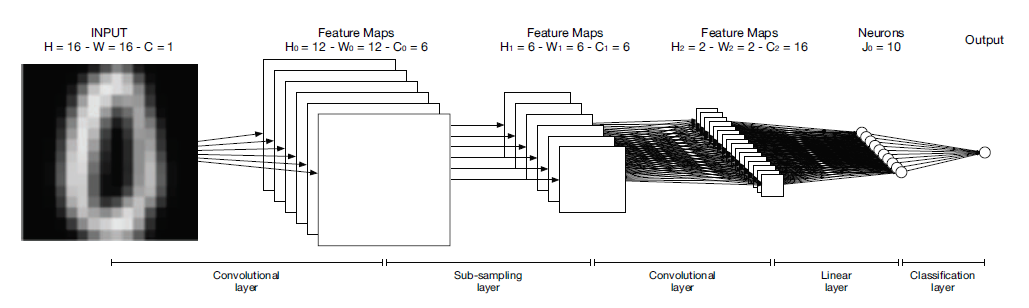
\includegraphics[width=0.45\textwidth]{01_images/Convolutional_Neural_Network_structure.PNG}}
	\caption{Convolutional Neural Network structure \cite{Bacis}.}
	\label{fig: Convolutional_Neural_Network_structure}
\end{figure}


\section{Conclusion}\label{Conclusion}
After introducing the audition to the topic and sate common definitions with simple scenarios two papers where chosen to present as example. The pipelined convolutional FPGA approach as well as the planetary rover application shows that FPGA show significant advantages in power efficiency and processing speed by 95x. 
In addition, the reader could gain a sense of what is it about when scientist talk about machine and deep learning and it allows to draw a line that for sure a small network one million connections is not an artificial intelligence (AI).


\begin{thebibliography}{00}
\bibitem{Learning} [1] “Learning | Definition of Learning by Merriam-Webster.” [Online]. Available: https://www.merriam-webster.com/dictionary/learning. [Accessed: 26-Sep-2018].
\bibitem{Caltech101} [2] “Caltech101.” [Online]. Available: http://www.vision.caltech.edu/Image\_Datasets/Caltech101/. [Accessed: 26-Sep-2018].
\bibitem{Neuron} [3] “Neuron | Definition of Neuron by Merriam-Webster.” [Online]. Available: https://www.merriam-webster.com/dictionary/neuron. [Accessed: 27-Sep-2018].
\bibitem{Schmidhuber} [4] J. Schmidhuber, “Deep learning in neural networks: An overview,” Neural Networks, vol. 61, pp. 85–117, Jan. 2015.
\bibitem{Hegde} [5] G. Hegde, Siddhartha, N. Ramasamy, V. Buddha, and N. Kapre, “Evaluating Embedded FPGA Accelerators for Deep Learning Applications,” in 2016 IEEE 24th Annual International Symposium on Field-Programmable Custom Computing Machines (FCCM), 2016, pp. 25–25.
\bibitem{Gankidi} [6] P. R. Gankidi and J. Thangavelautham, “FPGA architecture for deep learning and its application to planetary robotics,” in 2017 IEEE Aerospace Conference, 2017, pp. 1–9.
\bibitem{Bacis} [7] M. Bacis, G. Natale, E. Del Sozzo, and M. D. Santambrogio, “A pipelined and scalable dataflow implementation of convolutional neural networks on FPGA,” in 2017 IEEE International Parallel and Distributed Processing Symposium Workshops (IPDPSW), 2017, pp. 90–97.
%\bibitem{b5} R. Nicole, ``Title of paper with only first word capitalized,'' J. Name Stand. Abbrev., in press.
%\bibitem{b6} Y. Yorozu, M. Hirano, K. Oka, and Y. Tagawa, ``Electron spectroscopy studies on magneto-optical media and plastic substrate interface,'' IEEE Transl. J. Magn. Japan, vol. 2, pp. 740--741, August 1987 [Digests 9th Annual Conf. Magnetics Japan, p. 301, 1982].
%\bibitem{b7} M. Young, The Technical Writer's Handbook. Mill Valley, CA: University Science, 1989.
\end{thebibliography}
%\vspace{12pt}
%\color{red}
%IEEE conference templates contain guidance text for composing and formatting conference papers. Please ensure that all template text is removed from your conference paper prior to submission to the conference. Failure to remove the template text from your paper may result in your paper not being published.

\end{document}

%
%\section{Ease of Use}
%
%\subsection{Maintaining the Integrity of the Specifications}
%
%The IEEEtran class file is used to format your paper and style the text. All margins, 
%column widths, line spaces, and text fonts are prescribed; please do not 
%alter them. You may note peculiarities. For example, the head margin
%measures proportionately more than is customary. This measurement 
%and others are deliberate, using specifications that anticipate your paper 
%as one part of the entire proceedings, and not as an independent document. 
%Please do not revise any of the current designations.
%
%\section{Prepare Your Paper Before Styling}
%Before you begin to format your paper, first write and save the content as a 
%separate text file. Complete all content and organizational editing before 
%formatting. Please note sections \ref{AA}--\ref{SCM} below for more information on 
%proofreading, spelling and grammar.
%
%Keep your text and graphic files separate until after the text has been 
%formatted and styled. Do not number text heads---{\LaTeX} will do that 
%for you.
%
%\subsection{Abbreviations and Acronyms}\label{AA}
%Define abbreviations and acronyms the first time they are used in the text, 
%even after they have been defined in the abstract. Abbreviations such as 
%IEEE, SI, MKS, CGS, ac, dc, and rms do not have to be defined. Do not use 
%abbreviations in the title or heads unless they are unavoidable.
%
%\subsection{Units}
%\begin{itemize}
%\item Use either SI (MKS) or CGS as primary units. (SI units are encouraged.) English units may be used as secondary units (in parentheses). An exception would be the use of English units as identifiers in trade, such as ``3.5-inch disk drive''.
%\item Avoid combining SI and CGS units, such as current in amperes and magnetic field in oersteds. This often leads to confusion because equations do not balance dimensionally. If you must use mixed units, clearly state the units for each quantity that you use in an equation.
%\item Do not mix complete spellings and abbreviations of units: ``Wb/m\textsuperscript{2}'' or ``webers per square meter'', not ``webers/m\textsuperscript{2}''. Spell out units when they appear in text: ``. . . a few henries'', not ``. . . a few H''.
%\item Use a zero before decimal points: ``0.25'', not ``.25''. Use ``cm\textsuperscript{3}'', not ``cc''.)
%\end{itemize}
%
%\subsection{Equations}
%Number equations consecutively. To make your 
%equations more compact, you may use the solidus (~/~), the exp function, or 
%appropriate exponents. Italicize Roman symbols for quantities and variables, 
%but not Greek symbols. Use a long dash rather than a hyphen for a minus 
%sign. Punctuate equations with commas or periods when they are part of a 
%sentence, as in:
%\begin{equation}
%a+b=\gamma\label{eq}
%\end{equation}
%
%Be sure that the 
%symbols in your equation have been defined before or immediately following 
%the equation. Use ``\eqref{eq}'', not ``Eq.~\eqref{eq}'' or ``equation \eqref{eq}'', except at 
%the beginning of a sentence: ``Equation \eqref{eq} is . . .''
%
%\subsection{\LaTeX-Specific Advice}
%
%Please use ``soft'' (e.g., \verb|\eqref{Eq}|) cross references instead
%of ``hard'' references (e.g., \verb|(1)|). That will make it possible
%to combine sections, add equations, or change the order of figures or
%citations without having to go through the file line by line.
%
%Please don't use the \verb|{eqnarray}| equation environment. Use
%\verb|{align}| or \verb|{IEEEeqnarray}| instead. The \verb|{eqnarray}|
%environment leaves unsightly spaces around relation symbols.
%
%Please note that the \verb|{subequations}| environment in {\LaTeX}
%will increment the main equation counter even when there are no
%equation numbers displayed. If you forget that, you might write an
%article in which the equation numbers skip from (17) to (20), causing
%the copy editors to wonder if you've discovered a new method of
%counting.
%
%{\BibTeX} does not work by magic. It doesn't get the bibliographic
%data from thin air but from .bib files. If you use {\BibTeX} to produce a
%bibliography you must send the .bib files. 
%
%{\LaTeX} can't read your mind. If you assign the same label to a
%subsubsection and a table, you might find that Table I has been cross
%referenced as Table IV-B3. 
%
%{\LaTeX} does not have precognitive abilities. If you put a
%\verb|\label| command before the command that updates the counter it's
%supposed to be using, the label will pick up the last counter to be
%cross referenced instead. In particular, a \verb|\label| command
%should not go before the caption of a figure or a table.
%
%Do not use \verb|\nonumber| inside the \verb|{array}| environment. It
%will not stop equation numbers inside \verb|{array}| (there won't be
%any anyway) and it might stop a wanted equation number in the
%surrounding equation.
%
%\subsection{Some Common Mistakes}\label{SCM}
%\begin{itemize}
%\item The word ``data'' is plural, not singular.
%\item The subscript for the permeability of vacuum $\mu_{0}$, and other common scientific constants, is zero with subscript formatting, not a lowercase letter ``o''.
%\item In American English, commas, semicolons, periods, question and exclamation marks are located within quotation marks only when a complete thought or name is cited, such as a title or full quotation. When quotation marks are used, instead of a bold or italic typeface, to highlight a word or phrase, punctuation should appear outside of the quotation marks. A parenthetical phrase or statement at the end of a sentence is punctuated outside of the closing parenthesis (like this). (A parenthetical sentence is punctuated within the parentheses.)
%\item A graph within a graph is an ``inset'', not an ``insert''. The word alternatively is preferred to the word ``alternately'' (unless you really mean something that alternates).
%\item Do not use the word ``essentially'' to mean ``approximately'' or ``effectively''.
%\item In your paper title, if the words ``that uses'' can accurately replace the word ``using'', capitalize the ``u''; if not, keep using lower-cased.
%\item Be aware of the different meanings of the homophones ``affect'' and ``effect'', ``complement'' and ``compliment'', ``discreet'' and ``discrete'', ``principal'' and ``principle''.
%\item Do not confuse ``imply'' and ``infer''.
%\item The prefix ``non'' is not a word; it should be joined to the word it modifies, usually without a hyphen.
%\item There is no period after the ``et'' in the Latin abbreviation ``et al.''.
%\item The abbreviation ``i.e.'' means ``that is'', and the abbreviation ``e.g.'' means ``for example''.
%\end{itemize}
%An excellent style manual for science writers is \cite{b7}.
%
%\subsection{Authors and Affiliations}
%\textbf{The class file is designed for, but not limited to, six authors.} A 
%minimum of one author is required for all conference articles. Author names 
%should be listed starting from left to right and then moving down to the 
%next line. This is the author sequence that will be used in future citations 
%and by indexing services. Names should not be listed in columns nor group by 
%affiliation. Please keep your affiliations as succinct as possible (for 
%example, do not differentiate among departments of the same organization).
%
%\subsection{Identify the Headings}
%Headings, or heads, are organizational devices that guide the reader through 
%your paper. There are two types: component heads and text heads.
%
%Component heads identify the different components of your paper and are not 
%topically subordinate to each other. Examples include Acknowledgments and 
%References and, for these, the correct style to use is ``Heading 5''. Use 
%``figure caption'' for your Figure captions, and ``table head'' for your 
%table title. Run-in heads, such as ``Abstract'', will require you to apply a 
%style (in this case, italic) in addition to the style provided by the drop 
%down menu to differentiate the head from the text.
%
%Text heads organize the topics on a relational, hierarchical basis. For 
%example, the paper title is the primary text head because all subsequent 
%material relates and elaborates on this one topic. If there are two or more 
%sub-topics, the next level head (uppercase Roman numerals) should be used 
%and, conversely, if there are not at least two sub-topics, then no subheads 
%should be introduced.
%
%\subsection{Figures and Tables}
%\paragraph{Positioning Figures and Tables} Place figures and tables at the top and 
%bottom of columns. Avoid placing them in the middle of columns. Large 
%figures and tables may span across both columns. Figure captions should be 
%below the figures; table heads should appear above the tables. Insert 
%figures and tables after they are cited in the text. Use the abbreviation 
%``Fig.~\ref{fig}'', even at the beginning of a sentence.
%
%\begin{table}[htbp]
%\caption{Table Type Styles}
%\begin{center}
%\begin{tabular}{|c|c|c|c|}
%\hline
%\textbf{Table}&\multicolumn{3}{|c|}{\textbf{Table Column Head}} \\
%\cline{2-4} 
%\textbf{Head} & \textbf{\textit{Table column subhead}}& \textbf{\textit{Subhead}}& \textbf{\textit{Subhead}} \\
%\hline
%copy& More table copy$^{\mathrm{a}}$& &  \\
%\hline
%\multicolumn{4}{l}{$^{\mathrm{a}}$Sample of a Table footnote.}
%\end{tabular}
%\label{tab1}
%\end{center}
%\end{table}
%
%%\begin{figure}[htbp]
%%\centerline{\includegraphics{fig1.png}}
%%\caption{Example of a figure caption.}
%%\label{fig}
%%\end{figure}
%
%Figure Labels: Use 8 point Times New Roman for Figure labels. Use words 
%rather than symbols or abbreviations when writing Figure axis labels to 
%avoid confusing the reader. As an example, write the quantity 
%``Magnetization'', or ``Magnetization, M'', not just ``M''. If including 
%units in the label, present them within parentheses. Do not label axes only 
%with units. In the example, write ``Magnetization (A/m)'' or ``Magnetization 
%\{A[m(1)]\}'', not just ``A/m''. Do not label axes with a ratio of 
%quantities and units. For example, write ``Temperature (K)'', not 
%``Temperature/K''.
%
%\section*{Acknowledgment}
%
%The preferred spelling of the word ``acknowledgment'' in America is without 
%an ``e'' after the ``g''. Avoid the stilted expression ``one of us (R. B. 
%G.) thanks $\ldots$''. Instead, try ``R. B. G. thanks$\ldots$''. Put sponsor 
%acknowledgments in the unnumbered footnote on the first page.
%
%\section*{References}
%
%Please number citations consecutively within brackets \cite{b1}. The 
%sentence punctuation follows the bracket \cite{b2}. Refer simply to the reference 
%number, as in \cite{b3}---do not use ``Ref. \cite{b3}'' or ``reference \cite{b3}'' except at 
%the beginning of a sentence: ``Reference \cite{b3} was the first $\ldots$''
%
%Number footnotes separately in superscripts. Place the actual footnote at 
%the bottom of the column in which it was cited. Do not put footnotes in the 
%abstract or reference list. Use letters for table footnotes.
%
%Unless there are six authors or more give all authors' names; do not use 
%``et al.''. Papers that have not been published, even if they have been 
%submitted for publication, should be cited as ``unpublished'' \cite{b4}. Papers 
%that have been accepted for publication should be cited as ``in press'' \cite{b5}. 
%Capitalize only the first word in a paper title, except for proper nouns and 
%element symbols.
%
%For papers published in translation journals, please give the English 
%citation first, followed by the original foreign-language citation \cite{b6}.